\graphicspath{{chapters/4_implementación/figures/}}

\chapter{Implementación}\label{chap:implementation}

La primera decisión de relvancia en el proceso de desarrollo fue implementar el algoritmo en la GPU.
La principal razón para esto es el alto grado de paralelismo que la misma ofrece.
A su vez, el ducto raster, ampliamente implementado y optimizado en las GPUs, puede ser reutilizado.
Esto reduce los cálculos necesarios a la hora de generar una imagen.  

La programación en GPU precisa un lenguaje \textbf{motor}, una API de gráficos y un lenguaje de \textbf{sombreado}.
El lenguaje motor ejecuta en la CPU y es el que realiza y coordina las llamadas a funcionalidades de la GPU.
La API de gráficos es la que provee la interfaz que utiliza el lenguaje motor para comunicarse con la GPU.
La misma es una especificación que los fabricantes de las tarjetas de video deben implementar si deciden soportarla.
El lenguaje de sombreado es el que se utiliza para escribir los shaders, programas que ejecutan directo en la GPU y hacen uso del paralelismo que esta ofrece.

Como lenguaje motor se eligió \textbf{Rust}, un lenguaje de sistemas moderno multiparadigma.
Fue escogido debido a su gran comunidad, su amplia documentación y a su poderoso manejador de paquetes cargo.  
Se caracteriza por ser eficiente al permitir un acceso a primitivas de bajo nivel.
Además, provee abstracciones de costo cero lo cual mejora la experiencia de desarrollo.
Otra característica a mencionar es la seguridad de memoria que impide comportamientos indefinidos en tiempo de ejecución.

Se consideró a su vez C++ dado que es el lenguaje más popular para aplicaciones gráficas.  
Si bien ambos lenguajes presentan una eficiencia similar, el factor que más pesó en la decisión fue la presencia de un manejador de paquetes.
El mismo permitió instalar varias dependencias más rápido y cambiarlas a lo largo del ciclo de desarrollo cuando esto fue necesario.
En este caso, dada la implementación en la GPU, la eficiencia y el manejo de memoria es secundario. 

Como API de gráficos se eligió \textbf{OpenGL}, junto con el lenguaje de sombreado \textbf{GLSL}, el más usado para OpenGL, aunque este soporte otros lenguajes.
También fueron consideradas CUDA y Vulkan, pero se terminó por escoger OpenGL debido a la facilidad de desarrollo, el conocimiento previo del equipo y la facilidad de trabajo con \textit{compute shaders}.
Si bien Vulkan es una API más moderna, es conocida por ser más compleja que OpenGL y el equipo del trabajo no contaba con la suficiente experiencia para utilizarlo adecuadamente.
Esto hubiera llevado a mayores tiempos de desarrollo y no necesariamente a una implementación más eficiente.
CUDA suele usarse para cómputo de propósito general en la GPU, el cual hubo mucho, sin embargo, también fue utilizado el ducto raster, algo que CUDA no tiene.
Por esto se optó por utilizar los compute shaders de OpenGL para el cómputo de propósito general necesario.

El desarrolló se realizó en el sistema operativo \textbf{Linux} debido a los ambientes de desarrollo utilizados.
De igual manera, tanto Rust como OpenGL son multiplataforma, con lo que la aplicación es facilmente portable a otros sistemas operativos.

La arquitectura de la aplicación consta de tres paquetes: \textit{CLI}, \textit{Core} y \textit{Engine}.
\textit{Engine} contiene todas las abstracciones sobre OpenGL utilizadas, provee tipos como \textit{Transform}, \textit{Light}, \textit{Camera} que permiten manipular objetos en el espacio 3D.
\textit{Core} contiene todas las etapas y programas del algoritmo que han sido mencionados: voxelización, construcción del \textit{octree}, filtrado, actualización y el trazado de conos en si.
El paquete \textit{CLI} es el punto de entrada de la aplicación, procesa los argumentos pasados por linea de comandos y archivos de configuración y utiliza las funcionalidades expuestas por \textit{engine} y \textit{core} para crear un ambiente 3D y ejecutar el algoritmo.
Estos tres paquetes se muestran en la figura \ref{fig:overall_architecture}.

\begin{figure}
    \centering
    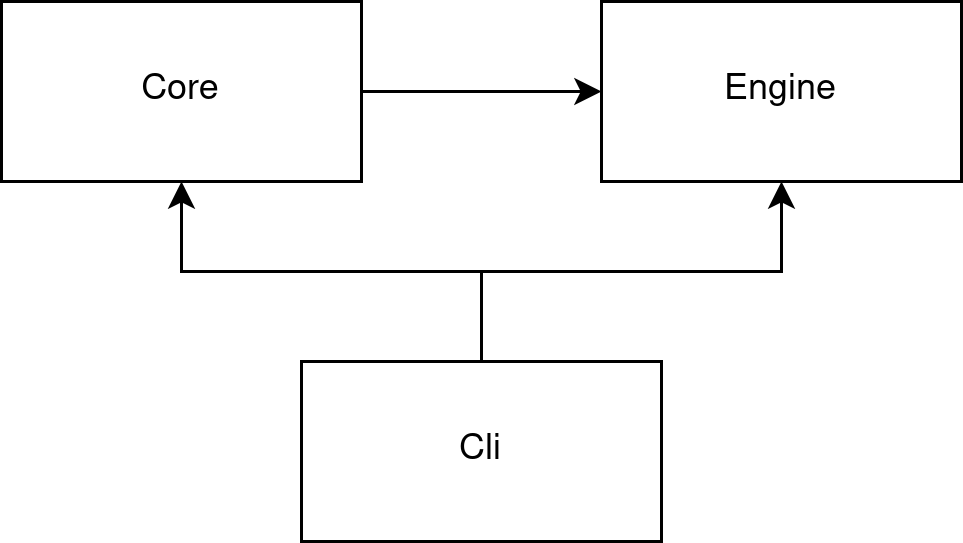
\includegraphics[width=\textwidth]{arquitectura_vct.png}
    \caption{Arquitectura de la aplicación}
    \label{fig:overall_architecture}
\end{figure}

En las siguientes secciones se verán más a detalle cada uno de estos paquetes.

\section{\textit{Engine}}

En este paquete, se implementaron las abstracciones usuales al trabajar con APIs de gráficos.

\textit{Transform} es un tipo que contiene la posición, rotación y escala de un objeto en la escena.
Esto simplifica el lidiar con matrices de traslación, rotación y escala por todo el programa, todo se maneja en el \textit{Transform}.

\textit{Camera} es el punto de vista del cual se renderiza toda la escena.
Se soportan tanto cámaras en perspectiva como ortogonales.

Debido al uso del ducto raster, la aplicación representa los modelos como mallas poligonales, distinto al trazado de rayos en el que se usan ecuaciones geométricas.
Para cargar estos modelos, se utilizó la librería \textit{tobj} \cite{tobj-crate}, que permite cargar archivos con extensión \textit{obj}.
Se usa una abstracción \textit{Model}, que contiene muchos \textit{Mesh}.

Para las luces, se soportan tanto luces direccionales como puntuales.
Estas luces tienen toda la lógica necesaria para que luego \textit{core} realice la inyección de fotones.

La estructura de árbol, los bricks, y todas las estructuras auxiliares, se almacenan en la memoria de la GPU.
Para esto, se ofrecen abstracciones sobre los distintos tipos de memorias y texturas de la GPU.
\textit{TextureBuffer}, \textit{Texture2D} y \textit{Texture3D} son ejemplos de estas, que manejan memoria lineal, bidimensional y tridimensional respectivamente.

Finalmente, se exponen las primitivas necesarias para crear una interfaz de usuario.
Luego, estas son usadas por \textit{core} para modificar parámetros del algoritmo.

\section{Core}

Este paquete es el corazón de la implementación, dado que es aquí donde se implementa el algoritmo.
Contiene la lógica de la voxelización, los tipos de datos del \textit{octree}, el trazado de conos y un menú para poder ajustar parámetros en tiempo de ejecución.

\subsection{Representación del \textit{octree}}

La forma de representar el árbol en GPU es con una textura lineal.
Esta textura que contiene los nodos toma el nombre de \textit{node pool}.
Cada téxel (píxel de textura) de esta textura es un puntero a otro nodo.
Se toma la convención de que cada grupo de 8 téxeles es un nodo, cada téxel es un puntero al hijo correspondiente.
Los primeros 4 téxeles representan una subdivisión con valor de $z$ menor mientras que los últimos 4 representan una con valor de $z$ mayor.
Dentro de cada grupo de 4, los primeros 2 son un valor menor de $y$ y los últimos uno mayor.
Dentro de los grupos de 2, el primero es menor $x$ y el último mayor.
Si un téxel tiene el valor $0$, entonces ese hijo del nodo no existe.
Si un téxel tiene un valor $x \not = 0$, entonces en la posición $x * 8$ comienza un nuevo nodo, que termina en $x * 8 + 7$.

Para representar los \textit{bricks}, se usa una gran textura 3D, llamada la \textit{brick pool}.
Cada brick es una sección de $3^3$ téxeles de esta textura 3D.
En cada uno de estos téxeles se almacenan valores de la escena, por ejemplo color.
Si otro valor quiere ser almacenado, por ejemplo la irradiancia, entonces se crea otra \textit{brick pool}.
Cada téxel dentro de un brick se llama vóxel, porque además de ser un píxel de textura, también es un píxel de volumen.

Cada nodo tiene asociado un brick, que es identificado únicamente por su índice.
Dado que los bricks existen en una textura 3D, la manera de identificarlos es con un vector de $\mathbb{R}^3$.
Para esto, se usa una función que convierte cada índice de $\mathbb{R}$ en un vector de $\mathbb{R}^3$.

\begin{figure}[h!]
    \centering
    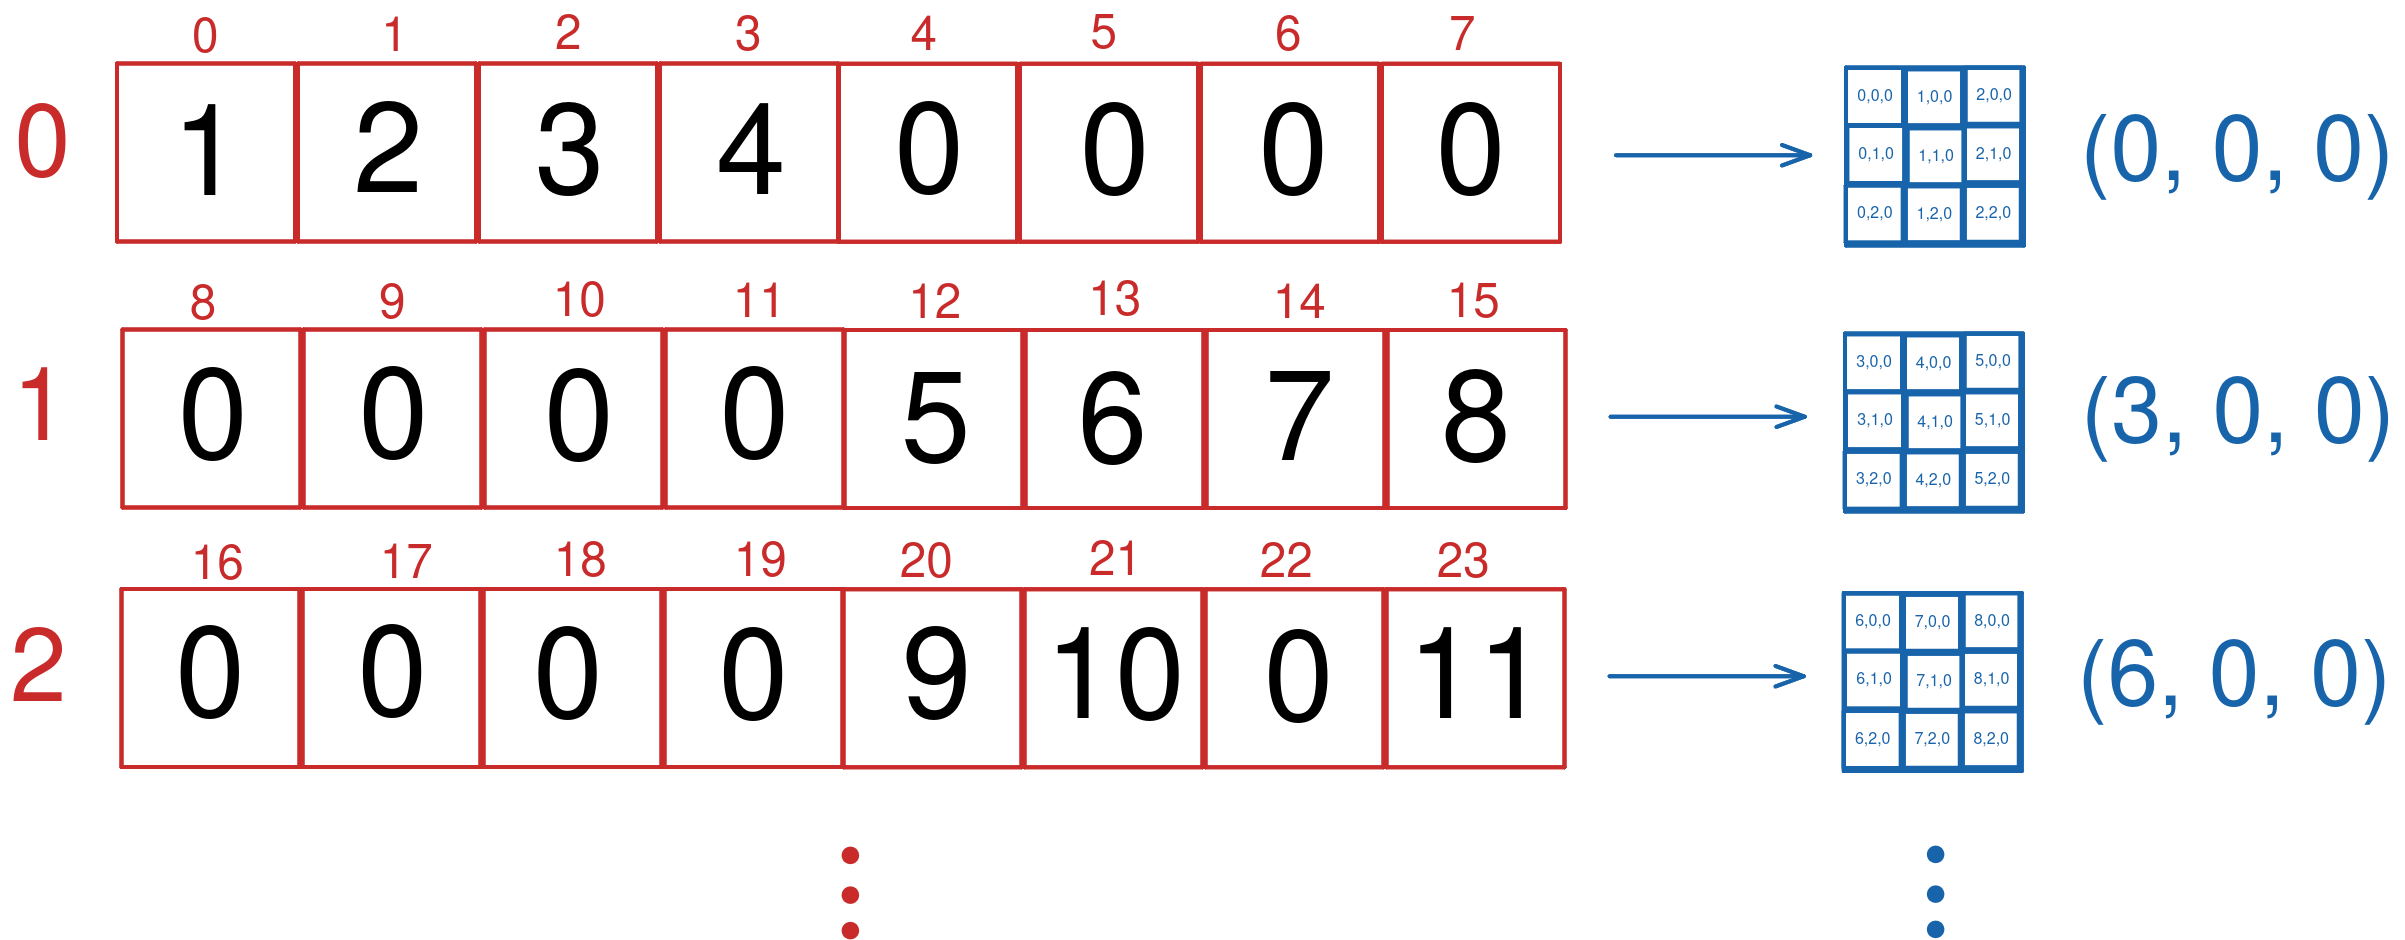
\includegraphics[width=\textwidth]{node-pool-example.png}
    \caption{Ejemplo node pool y brick pool}
    \label{fig:node_pool_example}
\end{figure}

En la figura \ref{fig:node_pool_example} se muestra un ejemplo de \textit{node pool} y \textit{brick pool}.
En este ejemplo, vemos que la \textit{node pool} está pintada de rojo, mientras que la \textit{brick pool} está pintada de azul.
Cada nodo de la \textit{node pool} está numerado en el margen izquierdo ($0, 1, 2$), está formado por $8$ téxeles, los pequeños números arriba de cada caja.
Los números dentro de cada téxel de un nodo son los índices del nodo hijo, que debe ser multiplicado por $8$ para conseguir el téxel correspondiente.

Al almacenar los valores en una textura 3D, conseguimos interpolación trilineal acelerada por el hardware de la GPU a la hora de tomar una muestra dentro de un brick.
Esto mejora la calidad de imagen.

\subsection{Menú}

A lo largo de la implementación, fue necesario depurar varios errores y correr pruebas.
Para esto, fue muy útil contar con una interfaz gráfica o menú para seleccionar varias opciones y poder ver valores de la GPU en tiempo real.
Se desarrolló este menú utilizando un paquete del ecosistema de Rust llamado \textit{Egui} \cite{egui}.

\textit{Egui} permite rápidamente crear una interfaz gráfica basada en ventanas que se renderiza junto con la aplicación en cada frame.
Es muy sencillo conectar valores del código a etiquetas en el menú y botónes en el menú a acciones.

El menú de la aplicación cuenta con varias ventanas, o submenúes, para ver valores, ajustar parámetros, y renderizar distintas imágenes.
Uno de submenúes más útiles para depurar es uno que muestra todos los nodos de la \textit{node pool}, permite buscarlos por índice y coordenadas, y visualizarlos en el espacio.

Esta se puede ver en la figura \ref{fig:node-positions-menu}.
En el menú se muestran todos los nodos de la node pool con su indice (0, 1, 2, ...) y sus coordenadas dentro de la escena (entre 0 y 255).
Al apretar cualquier nodo, se muestra en la escena un cubo delimitando la región de la escena representada por ese nodo.
Se pueden mostrar muchos nodos a la vez.

\begin{figure}
    \centering
    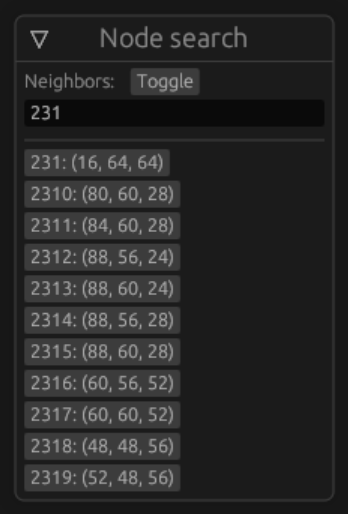
\includegraphics[width=.25\textwidth]{node-positions-menu.png}
    \caption{Menú de nodos}
    \label{fig:node-positions-menu}
\end{figure}

Este menú se puede filtrar, tanto por índice como por coordenadas, y se pueden mostrar los vecinos de cada nodo.

También se usó la interfaz gráfica para reportar los FPS que fueron usados en el capítulo \ref{chap:experiments}.

\section{CLI}

Este paquete es el punto de entrada de la aplicación.
Consta de un archivo \textit{main} que inicializa el contexto de OpenGL, la ventana de la aplicación, y utiliza \textit{engine} y \textit{core} para crear la escena con iluminación global.
También procesa varios tipos de archivos de configuración, que serán explicados a continuación.
Todos estos tipos de archivos contienen información en formato RON, por \textit{Rusty Object Notation}, una notación similar a JSON, \textit{JavaScript Object Notation}, pero diseñada específicamente para Rust.

\subsection{Archivo de configuración}

Cada ejecución de la aplicación carga un archivo de configuración que se encarga de definir ciertos parámetros.
Estos son la cantidad de vóxeles que se utilizarán, $256$, $512$ o $1024$; las dimensiones de la pantalla, entre otros.
A partir de esto, se inicializan otras variables, como la cantidad de niveles del octree, que es definida por la cantidad de vóxeles utilizados.
Estos parámetros son utilizados a lo largo de toda la aplicación, por lo que se usó el patrón singleton, creando un tipo \textit{Config}, que es inicializado una vez por \textit{CLI} y luego utilizado en el resto de la aplicación.

\subsection{Archivos de escena}

Para poder fácilmente cargar distintos modelos y probar el algoritmo en ellos, se creó un formato de archivos de escena.

En estos archivos se definen la lista de objetos y luces de la escena.
También se especifican listas de recursos para que los objetos referencien, modelos y materiales.
Estos recursos son cargados primero y los objetos pueden reutilizarlos sin necesidad de copiarlos.

Utilizando estos archivos, se pueden definir muchas escenas distintas para probar la implementación.

\subsection{Archivos de predeterminados}

Para poder iterar más rápido, se crearon archivos de predeterminados.
Estos archivos contienen valores predeterminados de opciones que cambian con el transcurso de la ejecución.
Por ejemplo, la posición de la cámara, qué tipo de imagen se está renderizando, qué nodos están siendo visualizados.
Estos archivos también pueden guardarse a partir del menú.
Son muy útiles cuando se está viendo algo en específico, y es necesario cambiar el código y recompilar, porque inmediatamente se vuelve al mismo lugar.
